\documentclass[a4paper]{article}

\usepackage{reportFormat}


\title{
	\Large {\sc Mech}4450 Aerospace Propulsion \\
	\Huge Major Assignment - Part 2
}

\author{
	Muirhead, Alex \\ \texttt{s4435062}
	\and
	Watt, Robert \\ \texttt{s4431151}
}

\date{\today}

\begin{document}

\pagenumbering{gobble}
\maketitle

% \tableofcontents

\vspace{10em}

\newpage


\section*{Nomenclature}
\pagenumbering{roman}


\newpage
\pagenumbering{arabic}

\section{Introduction}
The University of Queensland and our partners are developing a 3-stage, 93\% reusable, partially air-breathing small satellite launch system known as SPARTAN (Scramjet Powered Accelerator for Reusable Technology AdvaNcement). The SPARTAN mission profile is shown in figure 1. A rocket powered 1 st stage accelerates the vehicle stack to the minimum operating Mach number of the scramjet powered second stage (Mach 5). The 1 st
stage is then jettisoned and returns to base, and the scramjet accelerates the remainder of the vehicle to the scramjet cut-off Mach number of 10. A rocket powered 3 rd stage then separates from the second stage and accelerates the payload to orbit, while the second stage flies back to base.

The present SPARTAN design requires the second stage be fuelled with liquid hydrogen, since it is the most energetic fuel and gives the best propulsive performance. Even in its liquid form, however, hydrogen has low density and it is marginal whether the fuel tanks and required flight systems can be successfully packaged within the vehicle (this means it is possible, but even a small change in e. g. required wall thickness could cause the available volume to be insufficient). Furthermore, liquid hydrogen infrastructure is available at only a small subset of potential launch sites, which would greatly restrict where SPARTAN could be deployed. Both of these issues would be overcome if it was possible to fuel the scramjet with a denser hydrocarbon fuel, but this is challenging at high Mach numbers as hydrocarbon fuels have longer ignition and reaction times, and are less energetic. For this reason, the most promising hydrocarbon fuel for SPARTAN is ethylene (\(\ce{C2H4}\)) as it is the fastest reacting. UQ has had recent successes in experiments of supersonic combustion of ethylene in scramjet at Mach 8 [1, 2], but it is unknown if net thrust can be generated using ethylene fuel at Mach 10, where the time available for ignition and combustion is least. We would like you to be the engineering consultants who investigate this issue.

\section{Project Brief}
The task is to assess if the thrust generated by the scramjet powered second stage of the SPARTAN can exceed vehicle drag during Mach 10 flight (M = 10) if ethylene fuel is used. Whether the flow residence time within the engine is sufficiently long for reactions to proceed to completion is a key consideration, thus you modelling must incorporate the effects of finite rate chemistry. Part 1 of this project will focus on developing a chemistry module that takes the current temperature and pressure of the gas mixture as an input, internally computes the reaction rates and updates the mixture composition, the outputs the rate of heat released to the combustor. In Part 2 this module will be used within a quasi-one-dimensional cycle analysis to compute the performance of the scramjet.

\section{Methodology}\label{sec:methodology}
Combustion was modelled using the same model that was developed in part 1, however the temperature was calculated at each step along the solution from the heat released during combustion, rather than assuming a temperature profile ahead of time.

In order to calculate the temperature needed by the chemistry model, and also to calculate thrust, the total temperature and Mach number must be solved alongside the chemistry model. The additional equations to be solved are Eq.~\ref{eqn:dM2dx} and \ref{eqn:dTtdx}. Note that even though \(\ce{N2}\) doesn't react, it is included in the differential equations to be solved. Thus sums over reacting species become sums over all species, and scaling of reacting species' mass fractions to the mass fraction of \(\ce{N2}\) isn't needed.

\begin{align}\label{eqn:dM2dx}
    \frac{\partial M^2}{\partial x} =M^2 \frac{1 + \frac{\gamma_b - 1}{2}M^2}{1-M^2}\left( -\frac{2}{A} \frac{\partial A}{\partial x} + \frac{1 + \gamma_b M^2}{T_t}\frac{\partial T_t}{\partial x} + \frac{4 \gamma_b M^2 C_f}{D}\right)
\end{align}
\begin{align}\label{eqn:dTtdx}
    \frac{\partial T_t}{\partial x} = - \frac{1}{c_{pb}}\sum_i \frac{\partial Y_i}{\partial x}h_{f,i}^\circ
\end{align}
Where
\begin{align}\label{eqn:spatial_mass_fraction_gradient}
    \frac{\partial Y_i}{\partial x} = \mathcal{M}_i \left\lbrace \frac{1}{\sum_j \left[X_j\right]\mathcal{M}_j} \frac{\partial \left[X_i\right]}{\partial x} - \frac{\left[ X_i \right]}{\left(\sum_j \left[X_j\right]\mathcal{M}_j \right)^2 }\sum_j \mathcal{M}_j\frac{\partial \left[ X_j \right]}{\partial x} \right\rbrace
\end{align}
and 
\begin{align}\label{eqn:spatial_concentratoin_gradient}
    \frac{\partial \left[X_j\right]}{\partial x} = \frac{1}{v(x)}\frac{\partial \left[X_j\right]}{\partial t}
\end{align}
Where \(\frac{\partial \left[X_j\right]}{\partial t}\) is calculated using the chemistry model, and \(v(x)\) is the velocity of the gas \(x\)~m along the combustion chamber. This converts the time derivatives computed by the chemistry model into spatial derivatives needed to model the combustion. The velocity can be found using the Mach number of the flow at \(x\).
\begin{align}\label{eqn:v(x)}
    v(x) = M(x) \sqrt{\gamma_b R_b T(x)}
\end{align}
Since \(T_t(x)\) and \(M(x)\) is solved for at each time step, \(T(x)\) can be calculated using isentropic flow relations (Eq.~\ref{eqn:T(x)}). This is needed by the chemistry model, and to calculate \(v(x)\).
\begin{equation}\label{eqn:T(x)}
    T(x) = T_t(x) \left[ 1 + \frac{\gamma_b  - 1}{2}M(x)^2 \right]^{-1}
\end{equation}
Thus, using all the above equations, a system of ordinary differential equations can be solved to give the mass fraction of each species, total temperature and Mach number at each point along the combustor.
\begin{align}
    \frac{\partial}{\partial x} 
    \begin{bmatrix}
    \left[ \ce{C_2 H_4} \right] \\
    \left[ \ce{O_2} \right] \\
    \left[ \ce{H_2 O} \right] \\
    \left[ \ce{CO} \right] \\
    \left[ \ce{CO_2} \right] \\
    \left[ \ce{N_2} \right] \\
    T_t\\
    M^2
    \end{bmatrix}
    =
    \begin{bmatrix}
        f_0 \left(T_t, M^2, \left[ X_i \right]\right)\\
        f_1 \left(T_t, M^2, \left[ X_i \right]\right)\\
        f_2 \left(T_t, M^2, \left[ X_i \right]\right)\\
        f_3 \left(T_t, M^2, \left[ X_i \right]\right)\\
        f_4 \left(T_t, M^2, \left[ X_i \right]\right)\\
        f_5 \left(T_t, M^2, \left[ X_i \right]\right)\\
        f_6 \left(T_t, M^2, \left[ X_i \right]\right)\\
        f_7 \left(T_t, M^2, \left[ X_i \right]\right)
    \end{bmatrix}
\end{align}
Additionally, the density of the flow at each point along the combustor can be calculated from conservation of mass.
\begin{align}
    \rho(x) = \frac{\dot{m}}{v(x) A(x)}
\end{align}
This density can then be used to calculate the pressure at each point in the combustor using the ideal gas law.
\begin{align}
    P(x) = \rho(x) R T(x)
\end{align}

\section{Results and Discussion}
\subsection{Inlet Modelling}
The flight conditions of the scramjet can be used to calculate properties of the gas entering the scramjet. Given values for the freestream flight conditions are listed in Table.~\ref{tab:freestream values}. 
\begin{table}[H]
    \centering
    \begin{tabu} spread 0cm {X[-1,l]X[-1,c]X[-1,r]}
        \toprule 
        \rowfont[c]{\bfseries} Property & Symbol & Value \\
        \midrule 
        Mach Number & \(M_0\) & 10 \\
        Static Temperature & \(T_0\) & \SI{220}{\K} \\
        Dynamic Pressure & \(q_0\) & \SI{50}{\kPa} \\
        Specific Gas Constant & \(R\) & \SI{287}{\J\per\kg\per\K} \\
        \bottomrule 
    \end{tabu}
    \caption{Freestream flight conditions}
    \label{tab:freestream values}
\end{table}
Using the static temperature to calculate the speed of sound \(a_0^2 = \gamma R T_0\), and the flight Mach number, the velocity of gas entering the scramjet is given as:
\begin{equation}
    v_0 = M_0 \sqrt{\gamma R T_0} = \SI{2973}{\m\per\s}
\end{equation}
% \begin{align}
%     v_0 &= M_0 \sqrt{\gamma R T_0}\\
%     &= 10 \times \sqrt{1.4 \times 287 \times 220}\\
%     &=\SI{2973}{\m\per\s}
% \end{align}
The vehicle operates at constant dynamic pressure, given by the relation \(q_0 = \frac{1}{2}\rho_0v_0^2\). With velocity known, this can be rearranged to give the inlet density, and subsequently pressure from the ideal gas law. 
\begin{gather}
    \rho_0 = \frac{2 q_0}{v_0^2} = \SI{0.011}{\kg\per\m\cubed} \\
    p_0 = \rho_0 R T = \SI{714.4}{\Pa}
\end{gather}
% \begin{align}
%     \rho_0 &= \frac{2 q_0}{v_0^2}\\
%     &= \frac{2 \times 50 \times 10^3}{2973^2}\\
%     &= \SI{0.011}{\kg\per\m\cubed}
% \end{align}
% And the ideal gas law can be used to calculate the pressure at the inlet.
% \begin{align}
%     P_0 &= \rho_0 R T\\
%     % &= 0.011 \times 287 \times 220\\
%     &= \SI{714.4}{\Pa}
% \end{align}
The specific heat at constant pressure for the air fuel mixture can be calculated from the ratio of specific heats and gas constant determined from the CFD modelling of the inlet.
\begin{align}
    c_{pb} &= \frac{\gamma_b}{\gamma_b - 1}Rb\\
    % &= \frac{1.3205}{1.3205 - 1}\times 288.45\\
    % &= \SI{1188.45}{\J\per\kg\per\K}\\
    &= \SI{1.18845}{\kJ\per\kg\per\K}
\end{align}
The density of the air fuel mixture at the inlet to the combustor can be calculated using the ideal gas law.
\begin{align}
    \rho_{3b} &= \frac{P_{3b}}{RT_{3b}}\\
    &= \frac{\num{70.09e3}}{288.45 \times 1400}\\
    &= \SI{0.174}{\kg\per\m\cubed}
\end{align}
The area of the inlet to the combustor, \(A_3\), can be calculated from conservation of mass applied to the fully mixed air-fuel mixture at the combustor inlet.
\begin{align}
    A_3 = \frac{\dot{m}}{\rho_{3b} v_{3b}}
\end{align}
CALCULATE THE REMAINING FLOW STATES


\subsection{Combustor Modelling}
The system of equations presented in Section~\ref{sec:methodology} was solved using python (script provided in Appendix~\ref{app:code}). The engine performance at three different inflow temperatures; 1000~K, 1237.63~K, and 1400~K, was calculated. Plots of properties for each of these inflow temperatures along the combustor are plotted in Figs.~\ref{fig:properties_1000}, \ref{fig:properties_1238}, and \ref{fig:properties_1400} respectively. As can be seen, ignition doesn't occur at either 1000~K or 1237.63~K, however it does occur at 1400~K.

Figure \ref{subfig:stag_temp_1400} is particularly useful to see when ignition occurs (when the temperature reaches \(1.15 T_{t3}\), indicated on the graph). By determining when the stagnation temperature reaches the ignition temperature, it was possible to determine that ignition began 0.137~m along the combustor. Additionally, the point where the fuel runs out is evident in the sharp corner in the plot. The fuel runs out 0.142~m along the combustor. Thus the distance between ignition and burn out is 0.005~m, or 5~mm. The fuel burns extremely quickly once it ignites.

The state of the flow at the exit of the combustor is summarised in Table.~\ref{tab:combustor_exit_properties}.

\begin{table}[H]
    \centering
    \begin{tabu} spread 0cm {X[-1,c]X[-1,c]}
        \toprule 
                 Variable      &      Value       \\
        \midrule
              Mach Number &             2.82 \\
              Temperature & \SI{2925.27}{\K} \\
                 Pressure & \SI{34.27}{\kPa} \\
        Total Temperature & \SI{6649.83}{\K} \\
        \bottomrule
    \end{tabu}
    \caption{Combustor exit properties}
    \label{tab:combustor_exit_properties}
\end{table}

Combustion occurs within the first half of the combustor, and the second half of the combustor acts mostly as a nozzle, simply expanding the flow. Thus the combustor could be made shorter, so that the gas is expanded within the nozzle, where the area contour is designed specifically to expand the gas with mimumum losses, rather than for combustion.

RUN CODE WITH A SHORTER COMBUSTION CHAMBER AND SEE IF THRUST IS INCREASED. IF THRUST ISN'T INCREASED, THE ENGINE IS JUST MORE COMPACT.



\begin{widefigure}[10mm]
    \centering
    \begin{subfigure}[h]{0.49\linewidth}
        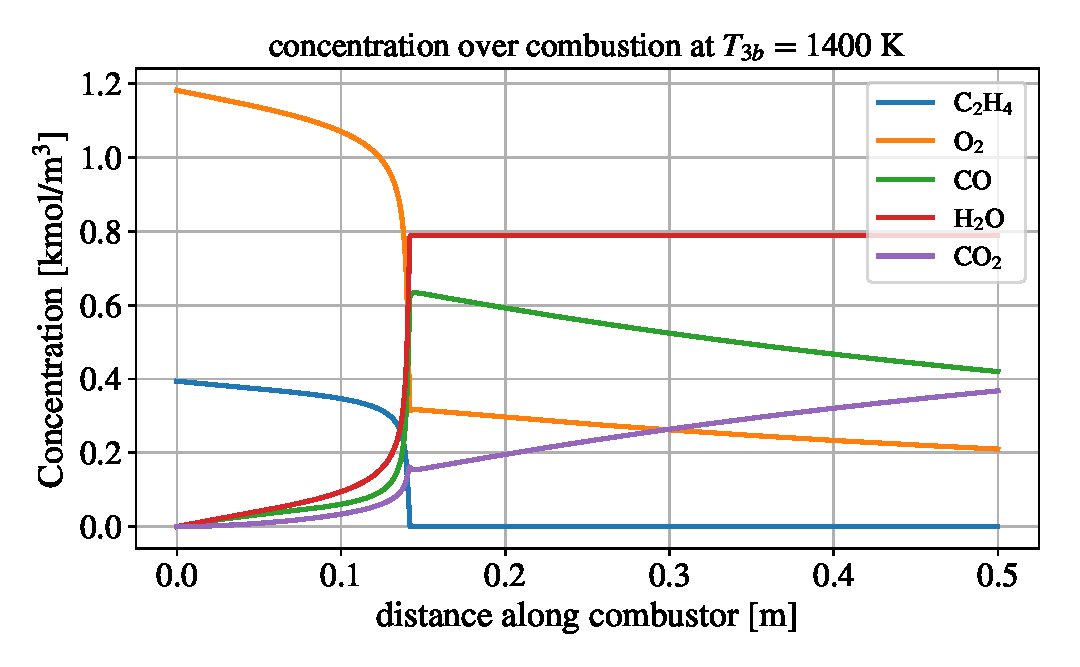
\includegraphics[width=\linewidth]{part_2_img/concentration_1400.pdf}
        \caption{Species Concentration}
        \label{subfig:concentration_1400}
    \end{subfigure}
    \begin{subfigure}[h]{0.49\linewidth}
        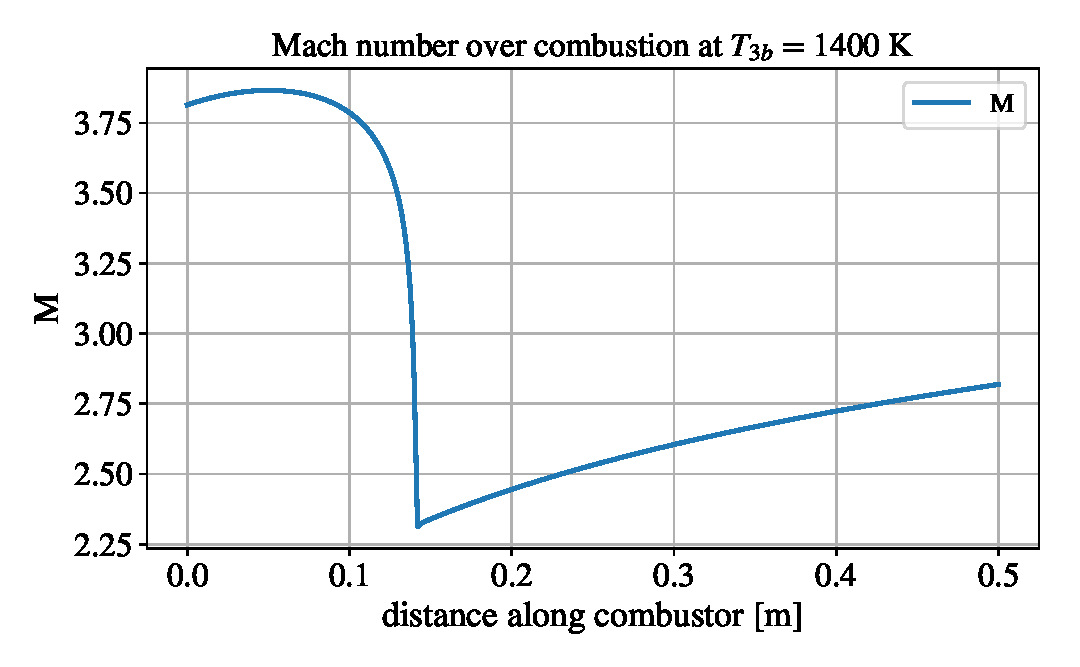
\includegraphics[width=\linewidth]{part_2_img/mach_1400.pdf}
        \caption{Mach number}
        \label{subfig:mach_1400}
    \end{subfigure}
    \begin{subfigure}[h]{0.49\linewidth}
        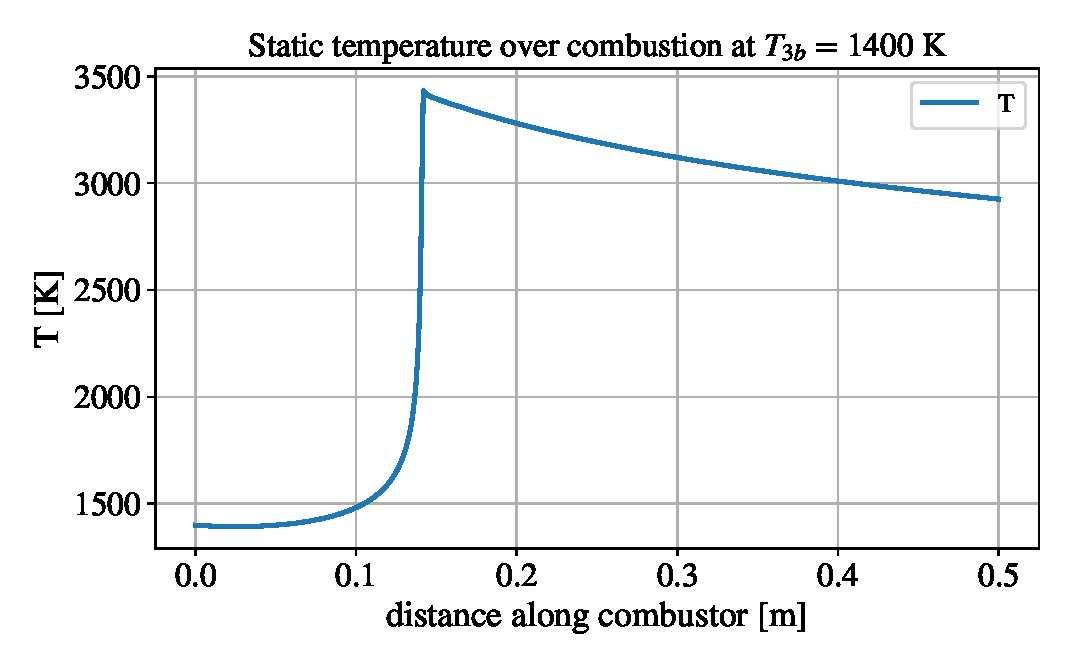
\includegraphics[width=\linewidth]{part_2_img/static_temp_1400.pdf}
        \caption{Static temperature}
        \label{subfig:temp_1400}
    \end{subfigure}
    \begin{subfigure}[h]{0.49\linewidth}
        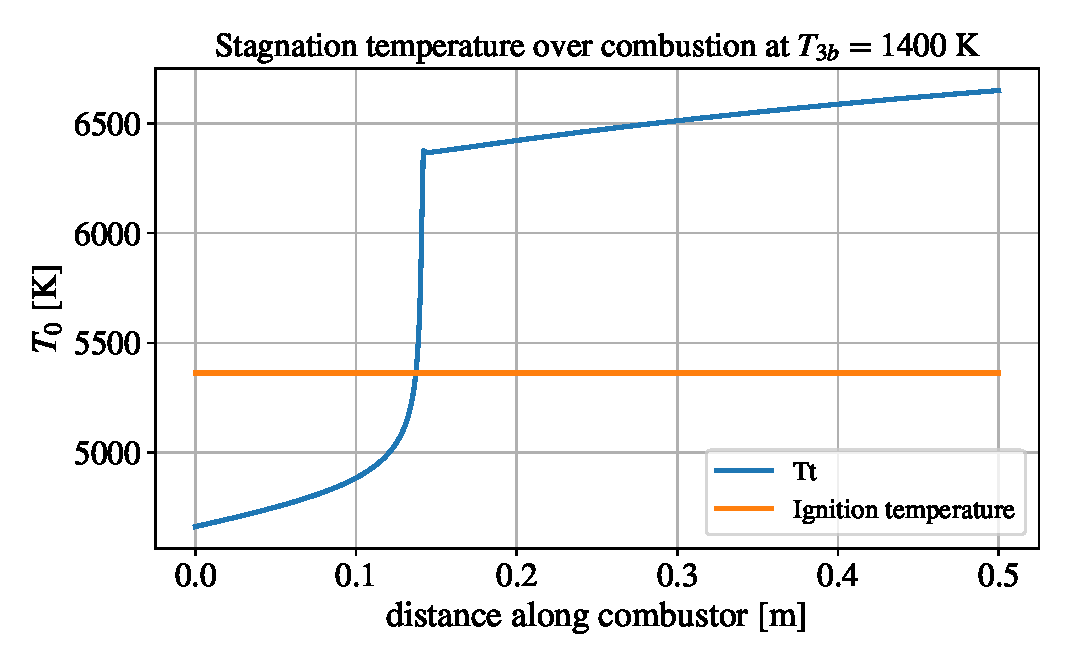
\includegraphics[width=\linewidth]{part_2_img/stag_temp_1400.pdf}
        \caption{Stagnation temperature}
        \label{subfig:stag_temp_1400}
    \end{subfigure}
     \begin{subfigure}[h]{0.49\linewidth}
        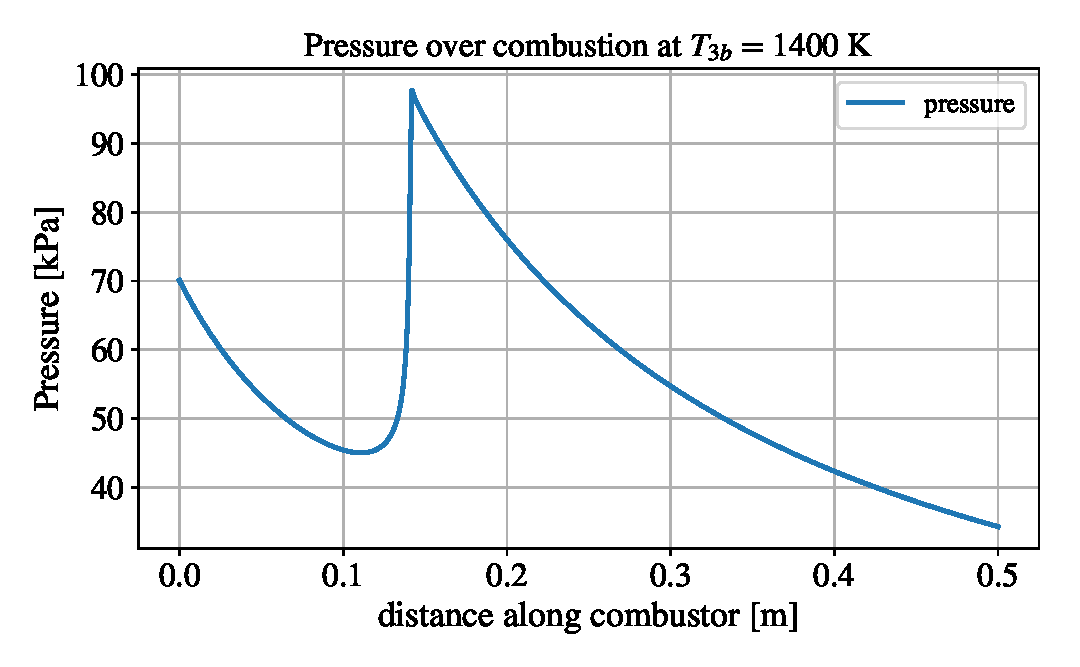
\includegraphics[width=\linewidth]{part_2_img/pressure_1400.pdf}
        \caption{Pressure}
        \label{subfig:pressure_1400}
    \end{subfigure}
    \caption{Properties over combustion at 1400~K}
    \label{fig:properties_1400}
\end{widefigure}

\subsection{Nozzle Modelling}
The flow state exiting the nozzle is summarised in Table.~\ref{tab:nozzle_exit_properties}.

\begin{table}[H]
    \centering
    \begin{tabu} spread 0cm {X[-1,l]X[-1,r]}
        \toprule \rowfont[c]{\bfseries} 
         Variable   &         Value         \\
        \midrule
        Mach Number &                  3.82 \\
        Temperature &      \SI{1492.64}{\K} \\
           Pressure &       \SI{2.14}{\kPa} \\
          Exit Area & \SI{2.51}{\m\squared} \\
             Thrust &     \SI{14573.61}{\N} \\
        \bottomrule
    \end{tabu}
    \caption{Nozzle exit properties}
    \label{tab:nozzle_exit_properties}
\end{table}


\subsection{Overall Performance and Discussion}
The overall performance of the scramjet is summarised in Table.~\ref{tab:performance}.

\begin{table}[H]
    \centering
    \begin{tabu} spread 0cm {X[-1,l]X[-1,r]}
        \toprule \rowfont[c]{\bfseries} 
             Variable     &           Value          \\ 
        \midrule
        Thrust per Engine &        \SI{14573.61}{\N} \\
          Specific Thrust & \SI{468.32}{\N\s\per\kg} \\
                     Drag &        \SI{29031.12}{\N} \\
                Net Force &        \SI{29263.31}{\N} \\
        \bottomrule
    \end{tabu}
    \caption{Scramjet Performance}
    \label{tab:performance}
\end{table}


\newpage
\appendix
\section{Plots}\label{app:other_plots}
\begin{figure}[H]
    \centering
    \begin{subfigure}[h]{0.49\linewidth}
        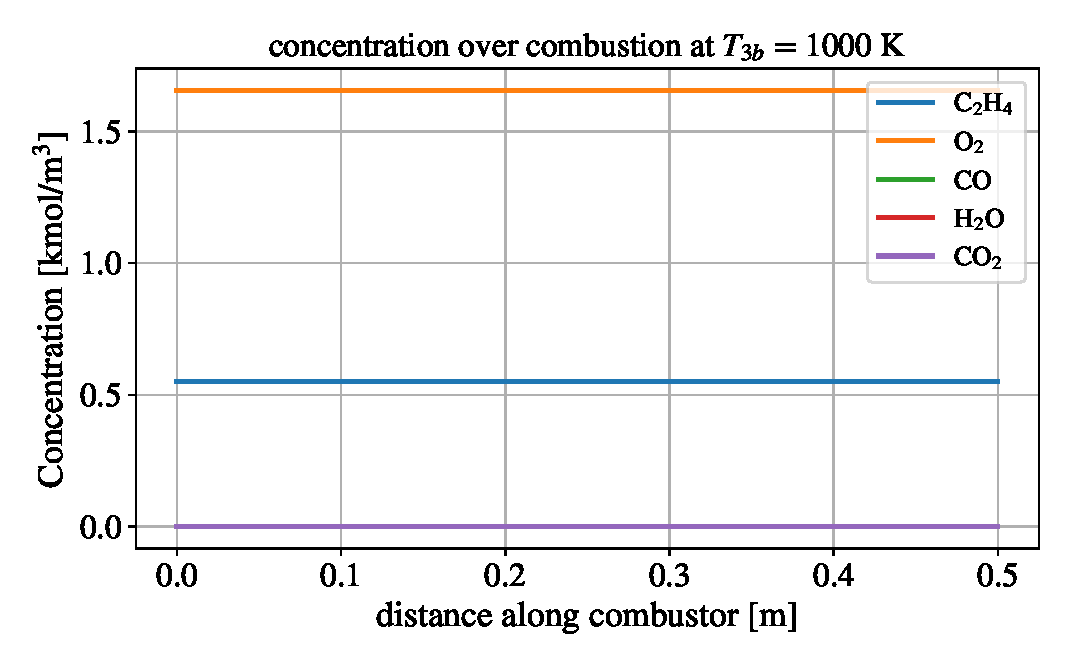
\includegraphics[width=\linewidth]{part_2_img/concentration_1000.pdf}
        \caption{Species Concentration}
        \label{subfig:concentration_1000}
    \end{subfigure}
    \begin{subfigure}[h]{0.49\linewidth}
        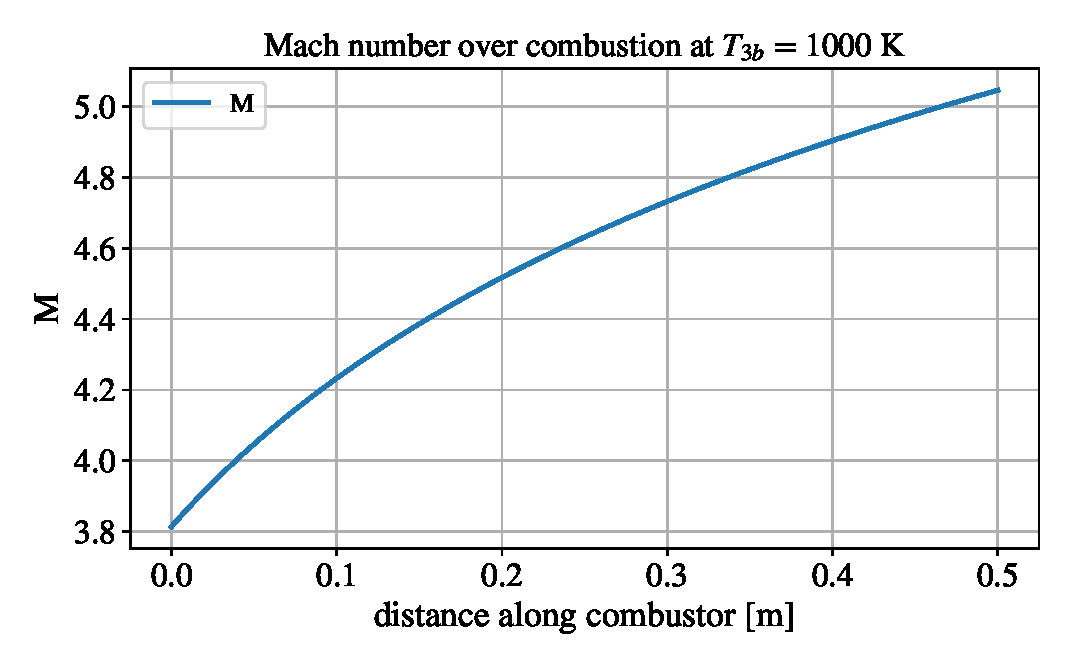
\includegraphics[width=\linewidth]{part_2_img/mach_1000.pdf}
        \caption{Mach number}
        \label{subfig:mach_1000}
    \end{subfigure}
    \begin{subfigure}[h]{0.49\linewidth}
        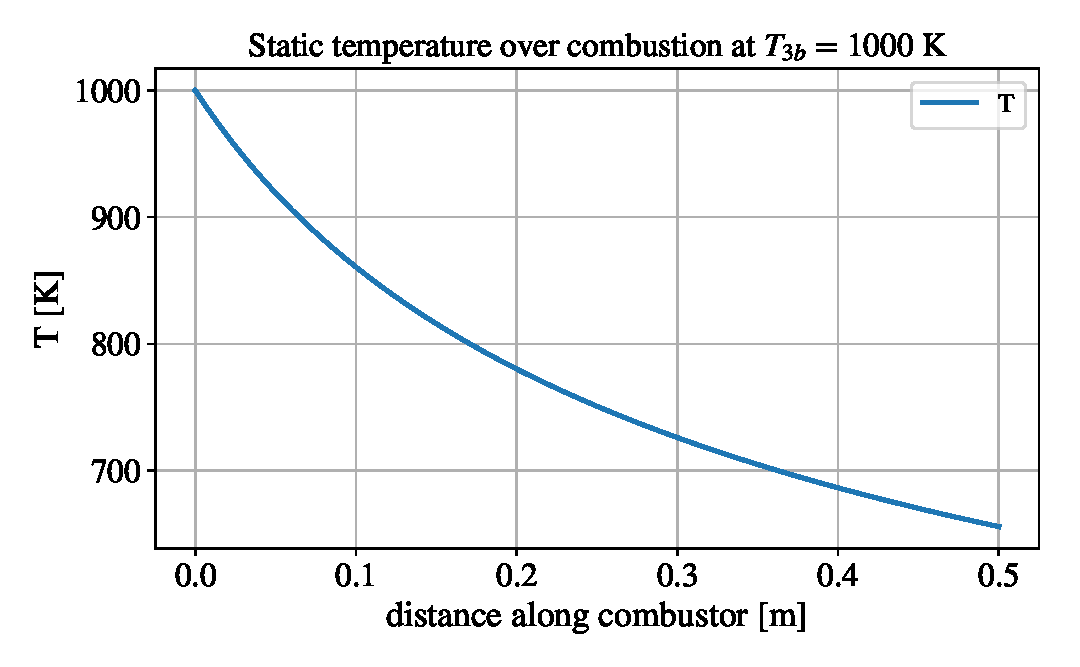
\includegraphics[width=\linewidth]{part_2_img/static_temp_1000.pdf}
        \caption{Static temperature}
        \label{subfig:temp_1000}
    \end{subfigure}
    \begin{subfigure}[h]{0.49\linewidth}
        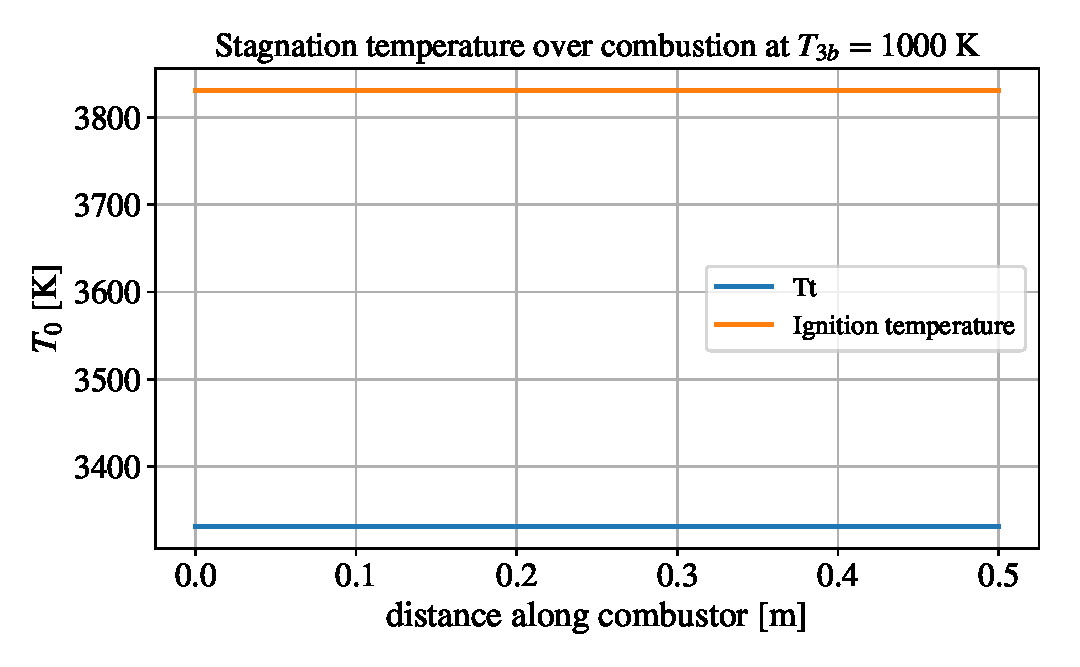
\includegraphics[width=\linewidth]{part_2_img/stag_temp_1000.pdf}
        \caption{Stagnation temperature}
        \label{subfig:stag_temp_1000}
    \end{subfigure}
     \begin{subfigure}[h]{0.49\linewidth}
        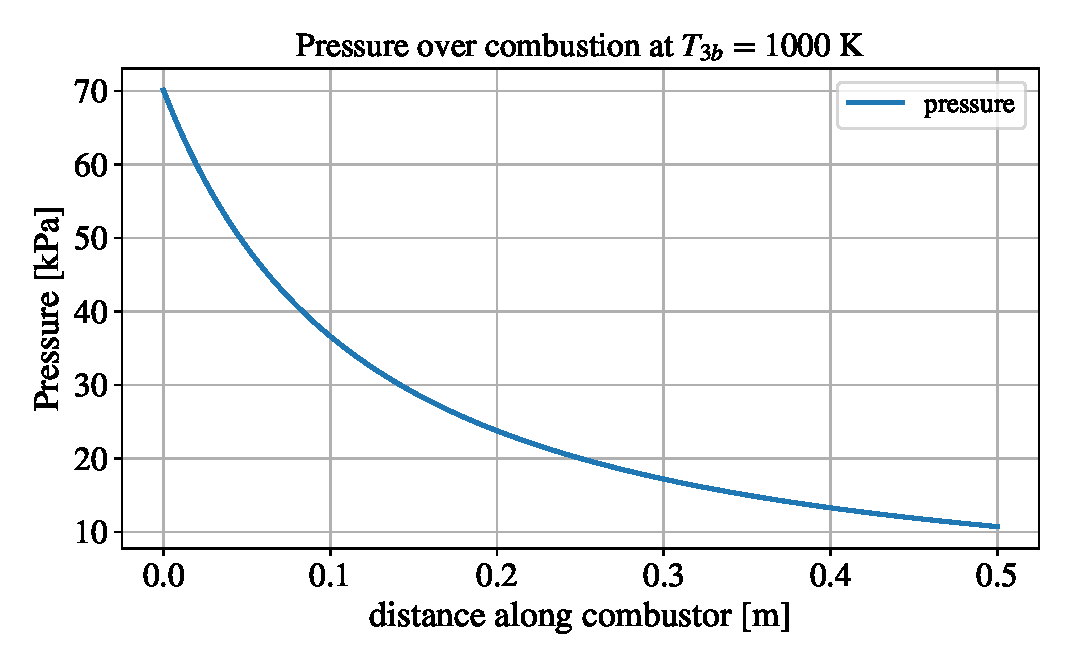
\includegraphics[width=\linewidth]{part_2_img/pressure_1000.pdf}
        \caption{Pressure}
        \label{subfig:pressure_1000}
    \end{subfigure}
    \caption{Properties over combustion at 1000~K}
    \label{fig:properties_1000}
\end{figure}

\begin{figure}[H]
    \centering
    \begin{subfigure}[h]{0.49\linewidth}
        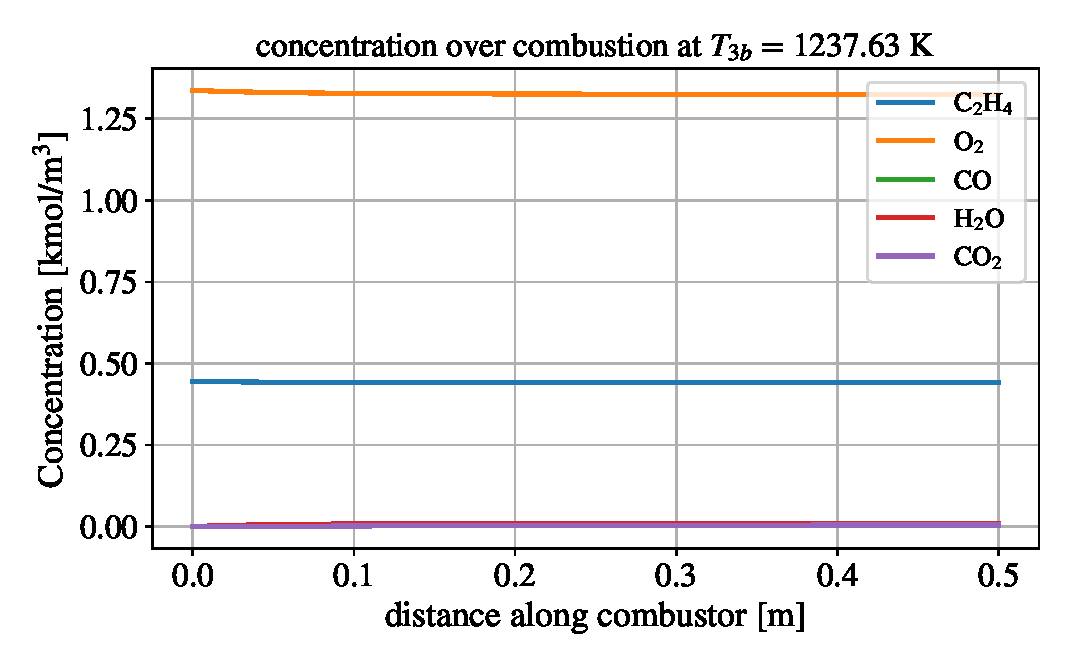
\includegraphics[width=\linewidth]{part_2_img/concentration_1238.pdf}
        \caption{Species Concentration}
        \label{subfig:concentration_1238}
    \end{subfigure}
    \begin{subfigure}[h]{0.49\linewidth}
        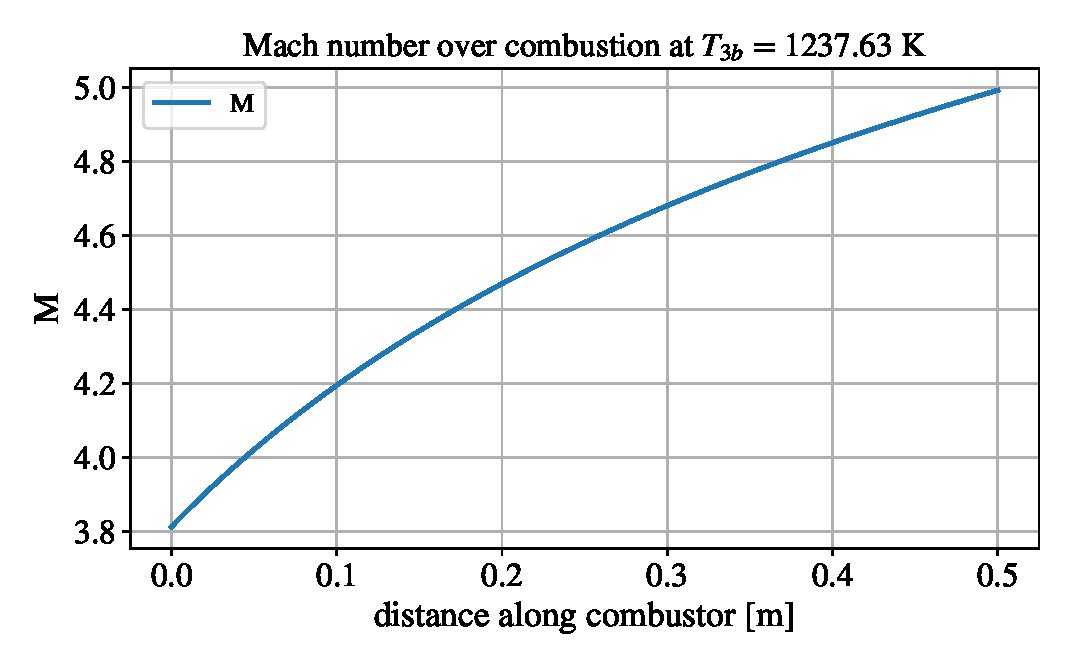
\includegraphics[width=\linewidth]{part_2_img/mach_1238.pdf}
        \caption{Mach number}
        \label{subfig:mach_1238}
    \end{subfigure}
    \begin{subfigure}[h]{0.49\linewidth}
        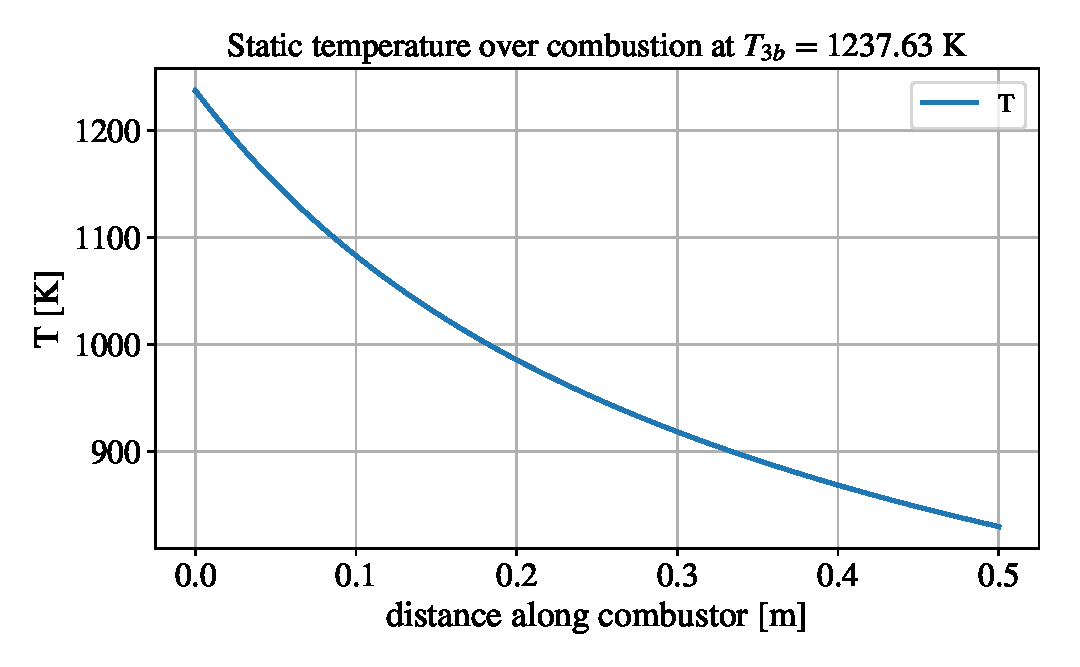
\includegraphics[width=\linewidth]{part_2_img/static_temp_1238.pdf}
        \caption{Static temperature}
        \label{subfig:temp_1238}
    \end{subfigure}
    \begin{subfigure}[h]{0.49\linewidth}
        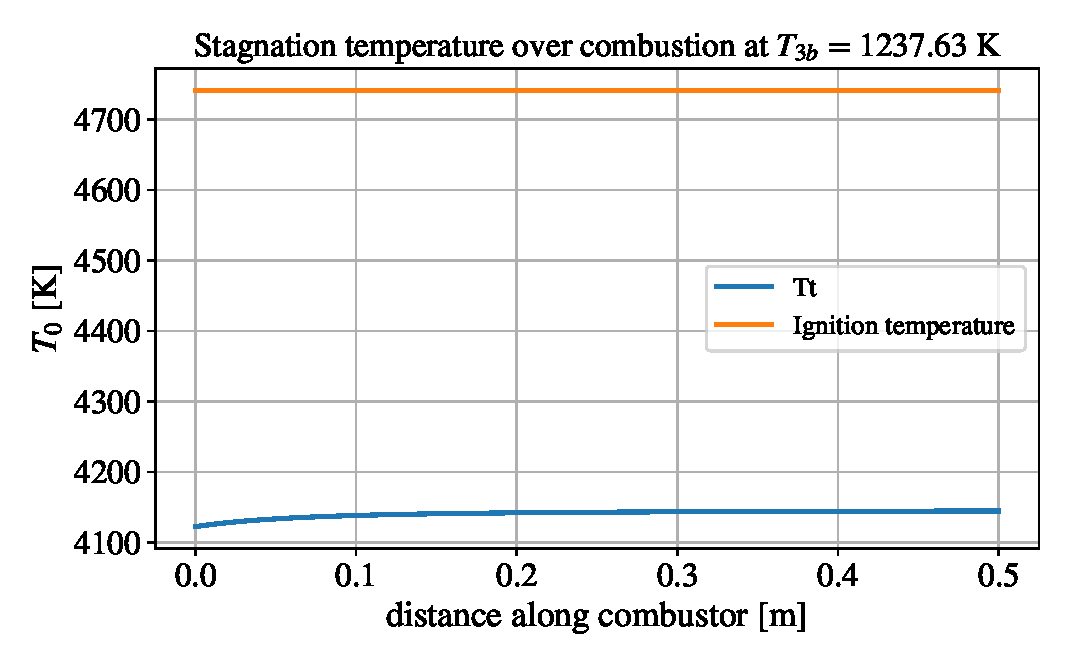
\includegraphics[width=\linewidth]{part_2_img/stag_temp_1238.pdf}
        \caption{Stagnation temperature}
        \label{subfig:stag_temp_1238}
    \end{subfigure}
     \begin{subfigure}[h]{0.49\linewidth}
        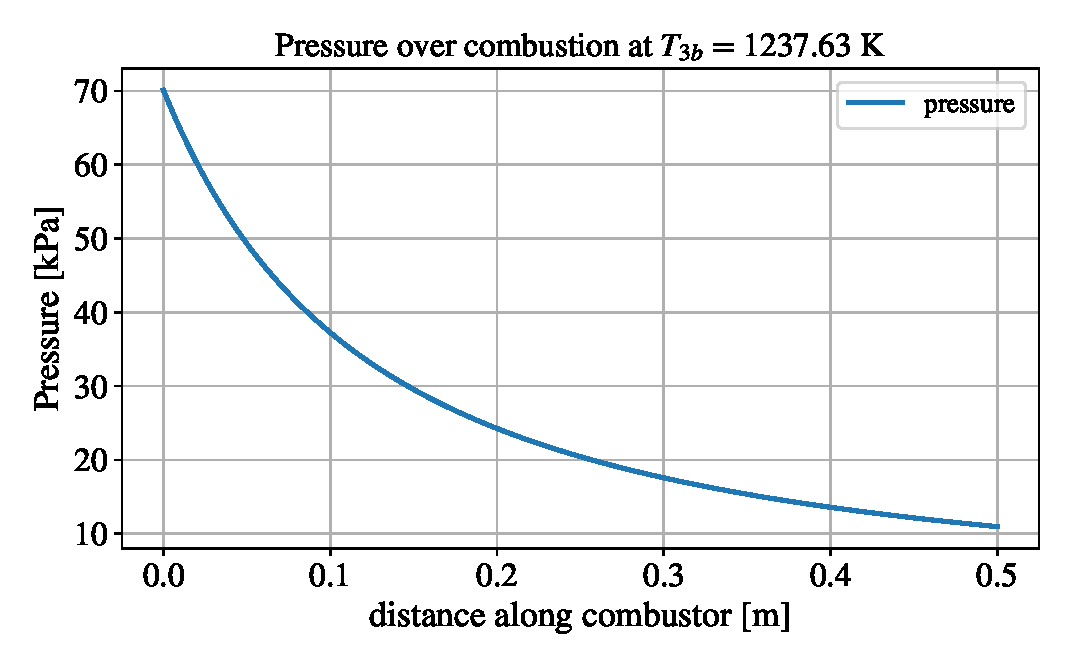
\includegraphics[width=\linewidth]{part_2_img/pressure_1238.pdf}
        \caption{Pressure}
        \label{subfig:pressure_1238}
    \end{subfigure}
    \caption{Properties over combustion at 1237.63~K}
    \label{fig:properties_1238}
\end{figure}

\newpage
\section{Python Solver}\label{app:code}
\inputminted[
	tabsize=4,
	obeytabs,
	fontsize=\footnotesize,
	frame=lines,
	framesep=0.5em,
	linenos
]{python}{code/part2IncludingN2.py}

\end{document}